\documentclass[paper=a4]{article}

\usepackage[english]{babel}
\usepackage[utf8]{inputenc}
\usepackage{amsmath,amssymb,latexsym,epsfig,graphics}
\usepackage[colorinlistoftodos]{todonotes}

\numberwithin{equation}{section}

\title{Approximations to the distributions of quadratic forms in normal variables}

\author{Sha Yu}

\date{\today}

\begin{document}
\maketitle

\section{Introduction}
Many test statistics are asymptotically equivalent to quadratic forms of normal variables,
which are further equivalent to the weighted sum of independent chi-square variables.

Consider the quadratic form $Q(X)=X'AX$, where X follows an n-dimensional multivariate normal distribution with mean vector $\mu_x$ and non-singular variance matrix $\Sigma$	, and A represents a $p \times p$ symmetric and nonnegative definite matrix. A problem of interest is to evaluate the probability  
\begin{align}
Pr(Q(X)>q)
\end{align}
By spectrual decomposition, a quadratic form can be converted to the weighted sum of independent chi-square variables. Let P be a $n \times n$ orthonormal matrix which converts $B={\Sigma}^{1/2}A{\Sigma}^{1/2}$ to the diagnoal form $\Lambda=diag(\lambda_1,...,\lambda_n)=PBP'$. Let $m=rank(A)$. We assume that $\lambda_1\geq...\geq\lambda_n\ge0$ and $\lambda_{m+1}=,..., =\lambda_n =0$ if $m<n$. Since $Y=P\Sigma^{-1/2}X$ is normally distributed with mean $P\Sigma^{-1/2}\mu_x$ and variance $I_n$, thus	
\begin{align}
Q=X'AX=Y'{\Lambda}Y=\sum_{r=1}^m\lambda_r\chi_{hr}^2(\delta_r)
\end{align}
where $h_r=1$, $\delta_r=\mu_{yr}^2$, and $\mu_{yr}$ is the ith component of $\mu_y$ for $r=1,...,m$.

Estimating the tail probability of $Q(x)$ arises in many statistical applications. The power analysis of a test procedure if the (asymptotic) distribution test statistic(e.g., Peason's chi-square statistic) takes the form Q(X). A famous example is the ChernoffLehmann test statistic for goodness-of-fit to a fixed distribution, which converges to quadratic form under the null (alternative) hypothesis (see, e.g., Moore and Spruill (1975) and Spruill (1976)). In time series analysis, Box-Pierece-Ljung portmanteau test statistic for lack of t in ARMA models converges in distribution to a weighted sum of non-central chi-square random variables under local alternatives. The quadratic forms are also the building
blocks for the commonly used F-statistics in ANOVA and regression.

It suggests the importance of determining (1.1) for quadratic forms in central and noncentral
normal variables in level and power studies. Thus (1.1) should be computed accurately
for quadratic forms in normal variables.
Unfortunately, for the probability density function (pdf) of weighted sum of independent chi-suqare variables, there is no known closed analytic expression yet except in some special cases. For instance, if $A\Sigma$ is idempotent matrix of rank p, then $Q(X)\sim \chi_{p,
	\lambda}^2$, where  $\lambda={{\mu_x}'}A\mu_x$.

Because the exact distribution of weighted sum of independent chi-square variables is difficult to obtain in general, various approximations to its distribution have been proposed. In section 2, we will illustrate five most popular appoximation approaches and their algorithms.

\section{Five appoximation approaches}
As mentioned, many methods have been proposed for the problem of (1.1). In this section, five most influential approxiamtion approaches will be illustrated.

\subsection{Imhof's Approximation}
Imhof derived this apporoximation using numerical integration to invert the characteristic function of $Q(X)$ in 1961. The charcteristic function of (1.1) is 
\begin{align}
\phi(t)=\sum_{r=1}^m(1-2i\lambda_rt)^{-\frac{h_r}{2}}exp(i\sum_{r=1}^m\frac{\delta_r^2\lambda_rt}{1-2i\lambda_rt})
\end{align}

The cumulative distribution function $F(x)$ of the variable Q defined by (1.1) can be obtained quite easily by straightforward numerical integration of an inversion formula. The standard inversion formula. Such a formula is implicit in work of Gurland (1948) and has been later derived explicitly by Gil-Pelaez (1951), namely
\begin{align}
F(x)=\frac{1}{2}-\frac{1}{\pi}\int_{0}^{\infty}t^{-1}g(e^{-itx}\phi(t))dt
\end{align}
where $g(z)$ denots the imaginary part of z and where the characteristic function $\phi(t)$ of $Q(X)$ is given by (2.1). Using the relations
\begin{center}
$arg[(1-ibt^{-y})]=gtan^{-1}(bt)$,  $|(1-ibt)^{-g}|=(1+b^2t^2)^{-\frac{1}{2}g}$,\\
$arg[exp(iat/(1-ibt))]=at/(1+b^2t^2)$,$|exp[iat/(1-ibt)]|=exp[-abt^2/(1+b^2t^2)]$,
\end{center}
one finds that for quardratic form Q of (1.1), equation (2.2) can be written after the substitution $2t=u$ is made,
\begin{align}
Pr(Q(X)>q)\approx\frac{1}{2}+\frac{1}{\pi}\int_{0}^{\infty}\frac{\sin\theta(u)}{u\rho(u)}du 
\end{align}	
where
\begin{center}
$\theta(u)=\frac{1}{2}\sum_{r=1}^m[h_r\arctan(\lambda_ru)+\delta_r^2\lambda_ru(1+\lambda_r^2u^2)^{-1}]-\frac{1}{2}qu$,
$\rho(u)=\prod_{r=1}^m(1+\lambda_r^2u^2)^{\frac{h_r}{4}}exp(\frac{\sum_{r=1}^m(\delta_r\lambda_ru)^2}{2(1+\lambda_r^2u^2)})$
\end{center}

This approximation is not easy to calculate but it can be very accurate and bounds on accuracy can be found. Also, the eigenvalues need be specified explicitly in order to apply this method, which is very time-consuming in the case that A is complex and high deminsional.

\subsection{Farebrother's Approximation}
Farebrother (1984) and Sheil and O'Muirchearatigh (1977), based on the results of Ruben (1962), exploit the fact that (1.1) can be written as an infinite series of an infinite series of centra chi-square distribtuions.
\begin{align}
Pr(Q(X)>q)=\sum_{k=0}^\infty c_k Pr(\chi_{2k+\tilde{h}}^2 >\frac{t}{\beta})  
\end{align}
For any $0< \beta <min(\lambda_1,...\lambda_m)$, where $\tilde{h}=\sum_{r=1}^mh_r$, $\gamma_r=1-\beta/\lambda_r$\\
$g_k=[\sum_{r=1}^mh_r\gamma_r^k+k\sum_{r=1}^m\delta_r\gamma_r^{k-1}(1-\gamma_r)]/2$
$ c_0=\prod{r=1}^m (\frac{\beta}{\lambda_r})^{\frac{h_r}{2}};exp(-\frac{\sum_{r=1}^m\delta_r}{2})$; $c_k=k^{-1}\sum_{k=o}^{k-r}g_{k-r}c_r$ for $k\geq1$. If the series is truncated after N terms, the truncation error is bounded by
\begin{center}
	$\sum_{k=N+1}^{\infty}c_k Pr(\chi_{2k+\tilde{h}}^2 > \frac{t}{\beta}) \leq \sum_{k=N+1}^\infty c_k=1-\sum_{k=1}^N c_k$
	\end{center}
	
	
This method also can be very accurate by bounding the error. However, it needs lots of computation and the eigenvalues need be specifed explicitly. In later comparison, we use this method as our golden standard.

\subsection{Pearson's three-moment central $\chi^2$ Approximation}
The Pearson (1959) approach was originally developed for approximating a non-central $\chi_l^2(\delta)$ distribution by a central $\chi_{l^*}^2$ distribution:
\begin{align}
Pr(\frac{\chi_l^2(\delta)-\mu_X}{\sigma_X}> t^*) \approx Pr(\frac{\chi_{l^*}^2-l^*}{\sqrt{2l^*}>t^*})
\end{align}
where $\chi_l^2(\delta)$ and $\chi_{l^*}^2$ have equal skewness. Imhof (1961) extended Pearson's method to the non-negative quadratic form:
\begin{align}
Pr(Q(X)>q)\approx Pr(\chi_{l^*}^2 >l^*+t^*\sqrt{2l^*})
\end{align}\\
where $l^*$ is determined so that Q(X) and $\chi_{l^*}^2$ have equal skewness. 
The cumulant generating function of Q(X) is given by Imhof (1961) 
\begin{align}
K(t) = -\frac {1}{2}\sum_{r=1}^m h_ilog(1-2t\lambda_r) + \sum_{r=1}^m \frac{\delta_r\lambda_rt}{1-2\lambda_rt}
\end{align}
The formula for the kth cumulant of Q(X) is 
\begin{align}
\kappa_k=2^{k-1}(k-1)!(\sum_{r=1}^m\lambda_r^kh_r+k \sum_{r=1}^m\lambda_r^k\delta_r)
\end{align}
It is uncessary to calculate the $\lambda_r$'s and $\delta_r$'s, since
\begin{center}
	$\sum_{r=1}^m \lambda_r^kh_i=trace(\Lambda^k)=trace((PBP')^k)=trace(B^k)=trace((A\Lambda)^k)$,
	$\sum_{r=1}^m\lambda_r^k\delta_r=\mu_y'\Lambda^k\mu_y=\mu_x'(A\Sigma)^{k-1}A\mu_x$.
\end{center}
The mean, standard deviation and skewness of Q(X) are given by
\begin{center}
	$\mu_Q=\kappa_1=c_1,  \sigma_Q=\sqrt{\kappa_2}=\sqrt{2c_2}, \beta_1=\frac{\kappa_3}{\kappa_2^{3/2}}=\sqrt{8}s_1$,
\end{center}
where $ c_k=\sum_{r=1}^m\lambda_r^kh_r+k \sum_{r=1}^m\lambda_r^k\delta_r$, $s_1=c_3/c_2^{3/2}$.

In Pearson's approximation, $l^*=1/s_1^2$. The accuracy of this method has been demonstrated in many empirical studies. Also, like other moment-cased approaches, this method does not involve inverting a matrix or calculating the eigenvalues of a matrix.

\subsection{ Liu-Tang-Zhang's four-moment non-central $\chi^2$ approximation}

LTZ proposed this method using a non-central $\chi_l^2(\delta)$ distribution to approximate the distribution of Q, thus
\begin{align}
Pr(Q(X)>q)\approx Pr(\chi_l^2(\delta) >t^*\sigma_X+\mu_X))
\end{align}
where 	$t^*=\frac{t-\mu_Q}{\sigma_Q}$, $\mu_x = l+\delta$, $\sigma_X=\sqrt{2(l+2\delta)}$. THe parameters $\delta$ and $l$ are determined so that the skewness of Q(X) and $\chi_l^2(\delta)$ are equal and the difference between the kurtosis of Q(X) and $\chi_l^2(\delta)$ is minimized.

From (2.7), the kurtosis of Q(X) is $\beta_2=\frac{\kappa_4}{\kappa_2^2}=12s_2$ and $s_2=c_4/c_2^2$. 

If $s_1^2 >s_2$, the minimum difference between the kurtosis Q(X) and $\chi_l^2(\delta)$ is 0 when $s_1^2-s_2=(1/a-s_1)^2$. Thus 
\begin{center}
$a=1/(s_1-\sqrt{s_1^2-s_2})$,   $\delta=s_1a^3-a^2$ and $l=a^2-2\delta$.
\end{center}

If $s_1^2\geq s_2$, the difference between the kurtosis of Q(X) and $\chi_l^2(\delta)$ is minimized when $a=1/s_1$. Thus
\begin{center}
	$a=1/s_1$, $\delta=s_1^3-a^2=0$ and $l=1/s_1^2=c_2^3/c_3^2$.
\end{center}

This method is closely related to Pearson's approximation and is equivalent to Pearson's approach when $s_1^2\geq s_2$. The better high-order moment approximation often improves the tail probability approximation in practice. And also this method does not involve inverting a matrix or calculating the eigenvalues of a matrix. In the next section, we will use a simulation study to show that the actual approximation error of this method is usually much smaller than that of Pearson's approximation.

\subsection{Kuonen's saddle point approximation}
By contrast to the Pearson's method, this method uses the entire cumulant generating function (2.7).
\begin{align}
Pr(Q(X)>q)\approx 1-\Phi(w+\frac{1}{w}log(\frac{v}{w}))
\end{align}
where 
\begin{center}
$w=sign(\hat{\xi})[2(\hat{\xi}q-K(\hat{\xi}))]^{\frac{1}{2}}$,  $v=\hat{\xi}(K^{''}(\hat{\xi}))^{\frac{1}{2}}$
\end{center}
and $\hat{\xi}=\hat{\xi}(q)$ is the saddle point which satisfies the equation $K^{'}(\hat{\xi})=q$;
$K'(\xi)$ and $K^{''}(\xi)$ are the first and second derivatives of $K(\xi)$ with respect to $\xi$.

Saddle point method gives high accuracy and is very easy to compute. However, the eigenvalues must be specified explicitly.

\section{Numerical examples simulation}

We consider five quadratic forms, which are defined in table 1.
	\begin{center}	
	\begin{tabular}{l}\hline\\
		$Q_1= 0.5\chi_1^2(1)+0.4\chi_2^2(0.6)+0.1\chi_1^2(0.8)$\\
		$Q_2= 0.9\chi_1^2(0.2)+0.1\chi_2^2(10)	$	\\
		$Q_3= 0.1\chi_1^2(0.2)+0.9\chi_2^2(10)	$	\\
		$Q_4= 0.5\chi_1^2(1)+0.4\chi_2^2(0.6)+\sum_{r=1}^{10}0.01\chi_r^2(0.8)$		\\
		$Q_5=\chi_1^2(1.0)+(0.6)^4\chi_1^2(7.0)$\\
        \hline	
		\end{tabular}
	\\
	Table 1
	\end{center}
	
The quadratic form $Q_1$ is inspired from Liu et al.(2009). $Q_2$ is a quadratic form with small weight assigned to the chi-square term with large non-centralility parameter. $Q_3$ is a quadratic form with large weight assigned to the chi-square term with large non-centralility parameter. These two quadratic forms are designed to check wether the weight and non-centralility parameter will affect the accuracy of approximation. $Q_4$ is a modification of $Q_1$. We decomposited the last term into 10 chi-square variables with same weight 0.01 and different degrees of freedoms. By comparing the results of $Q_1$ and $Q_4$, we want to check whether the quantity of chi-square variables will have an efffect on the performance of different approximation approaches. $Q_5$ is inspired from the asymptotic distribution of Box-Pirce-Ljung portmanteau test statistic, which is widely used in time series analysis. If a time series follows a ARMA model with parameter $\alpha$, then the Box-Pierce-Ljung portmanteau test statitic asympototically follows the quadratic form $\chi_{m-1}^2+\alpha^{2m}\chi_1^2$. We set $m=2$, $\alpha=0.6$.

For each quadratic form,we simulated 101 different q values. For $Q_1$, $Q_2$, $Q_4$ and $Q_5$, the sequence of q is from 1 to 11 with increment 0.1. To breifly analize the results, we only include the results of  $q=2,4,6,8,10$ in the absolute error table and relative error table. For $Q_3$, the sequence of q is from 1 to 20 with increment 0.2. The reason that the range of t is different for $Q_3$ is that when $t=10$, the value of (1.1) of quadratic form $Q_3$ is approximate 0.4, which is still quite large. So we extended the range of q values to make the analysis have more realistic meaning. We used  all simulated points to contruct qq plot. The results of these five quadratic forms in five approaches were presented in the next section.

\begin{center}	
	\begin{tabular}{l}
		\hline\\
		
		$imhof(q, \lambda, h, \delta ,epsabs = 10^{-6}, epsrel = 10^{-6})$\\
		$farebrother(q, \lambda, h, \delta ,epsabs = 10^{-6}, eps = 10^{-6})$\\
		$liu(q, \lambda, h)$\\
		\hline	
		\end{tabular}	\\
		Table 2
\end{center}	

The computations of Farebrother's method, Imhof's method and LTZ's method were all performed using R package CompQuadForm developed by P.Lafaye in 2015 and the results were identical with a precision of $10^{-6}$. The commands were presented in Table 2. Note that although LTZ's approximation does not involve calculating the eigenvalues of $Q(X)$, these values still need be specified explicitly in order to use this R package.


For Pearson's approach and Saddle point approach, the R demos were programmed according to their algorithms. R codes were presented in Figure 1 and Figure 2. We just used $Q_1$ as an example.
\begin{figure}[h]
	\begin{center}
%\graphicspath{{C:/Users/riyi/Desktop/yusha/STAT-5123/project}}
%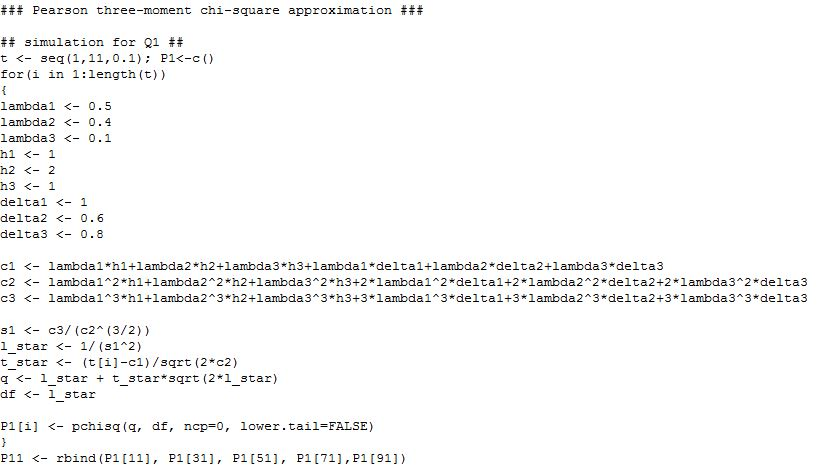
\includegraphics[width=\textwidth]{Pearson}
\caption{R demo of Pearson's approximation}
\end{center}
\end{figure}

\clearpage
\begin{figure}[h]
	\begin{center}
%	\graphicspath{{C:/Users/riyi/Desktop/yusha/STAT-5123/project}}
%	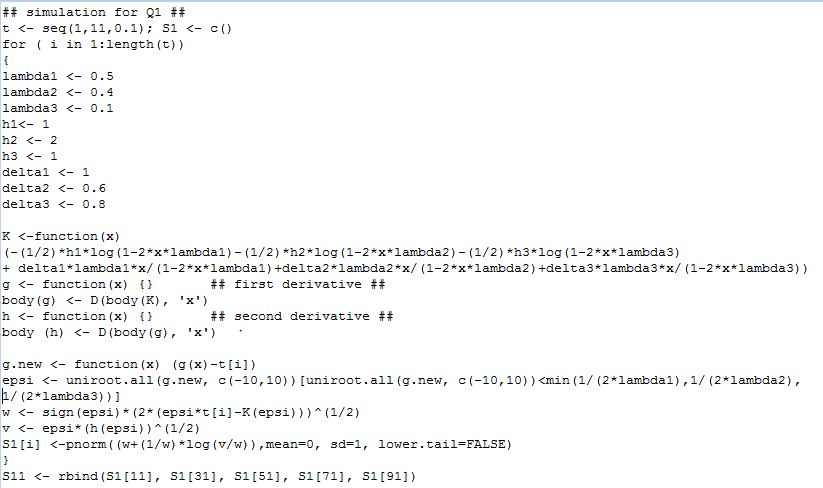
\includegraphics[width=\textwidth]{Saddle}
	\caption{R demo of Saddle point approximation}
\end{center}
\end{figure}


\section{Comparisons and discussion}

\textbf{Table 3}
\\*
\begin{small}
The column \texttt{AE\_I} gives the absolute errors of Imhof 's approximation compared to Farebrother's approximation. The column \texttt{AE\_P} gives the absolute errors of Pearsons's three-momoent center $\chi^2$ approximation compared to Farebrother's approximation. The column \texttt{AE\_L} gives the absolute errors of LTZ's four approximation compared to Farebrother's approximation. The column \texttt{AE\_S} gives the absolute errors of Saddle point approximation compared to Farebrother's approximation. 
\end{small}

\begin{center}
%		\graphicspath{{C:/Users/riyi/Desktop/yusha/STAT-5123/project}}
%		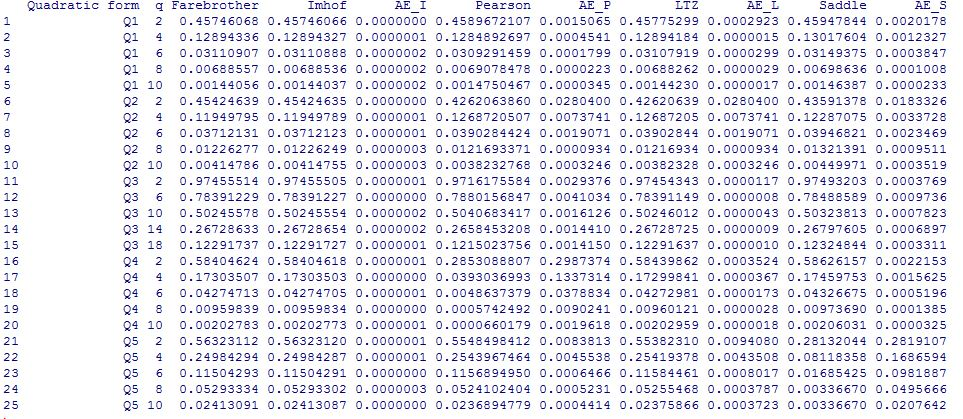
\includegraphics[width=\textwidth]{table1}
\end{center}

\clearpage
\begin{small}
	\setlength{\parindent}{0cm}
\textbf{Table 4}

The column \texttt{RE\_I} gives the relative error of Imhof 's approximation compared to Farebrother's approximation. The column \texttt{RE\_P} gives the relative errors of Pearsons's three-momoent center $\chi^2$ approximation compared to Farebrother's approximation. The column \texttt{RE\_L} gives the relative errors of LTZ's four approximation compared to Farebrother's approximation. The column \texttt{RE\_S} gives the relative errors of Saddle point approximation compared to Farebrother's approximation. 
\end{small}

\begin{center}
%	\graphicspath{{C:/Users/riyi/Desktop/yusha/STAT-5123/project}}
%	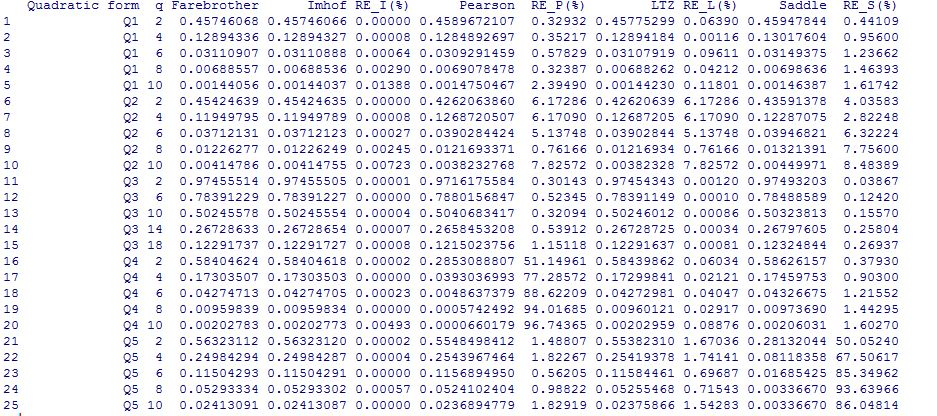
\includegraphics[width=\textwidth]{table2}
\end{center}

Our numerical examples demonstrate that Farebrother's approximation and Imhof's approximation differ very little. The accuracy of Pearon's approximation is quite good except for $Q_4$. LTZ's method yields better approximation than Pearson's method except $Q_2$. Since for quadratic form $Q_2$, it satisfies the condition that $s_1^2\leq s_2$, under which case, the LTZ's approximation and Pearson's approximation are the same as we illustrated in section 2. Saddle point approximation also gives high accuracy but overally it is not as good as LTZ's method. Pearson's approximation, LTZ's approximation and Saddle point approximation yield more errors when used to calculate tail probability of $Q_2$ compared to other quadratic forms.

We now discuss the results in more details. To check whether the weight and scale of non-centralility parameter have effect on the accuracy among different approaches, we contructed qqplots of $Q_2$ and $Q_3$ with y axes the results of Farebrother's approximation as in Figure 3. We can conclude that both Pearson's approximation and LTZ's approximation yield high accuracy in the case that the chi-square term with large non-centralility parameter has large weight.

To check whether the quantity of chi-square variables influents the accuracy of approximation, we contructed a qqplot comparing $Q_1$ and $Q_4$ as presented in Figure 4. The results indicate that Pearson's approximation performs poorly if the quantity of chi-square variable is large. Both LTZ's approximation and Saddle point appoximation yield high accuracy for these two quadratic forms.

A qqplot of the results of $Q_5$ is also contructed as presented in Figure 5. We could conclude that all methods yeild high accuracy.
\begin{figure}
	\begin{center}
%		\graphicspath{{C:/Users/riyi/Desktop/yusha/STAT-5123/project}}
%		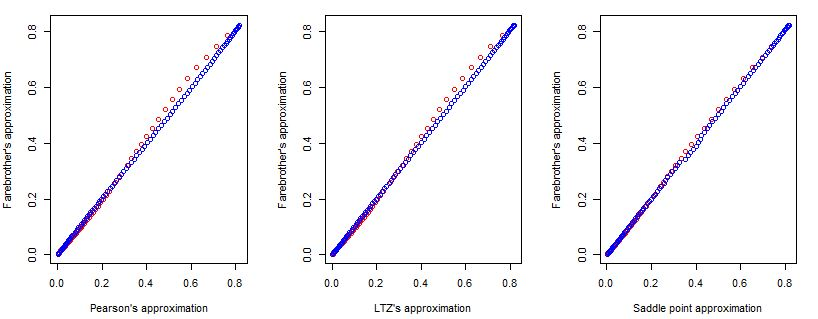
\includegraphics[width=\textwidth]{Q2&Q3}
		\title{Figure 3: qq plot of $Q_2$(red points) and $Q_3$(blue points)}
	\end{center}
\end{figure}
\begin{figure}[h]
	\begin{center}
%		\graphicspath{{C:/Users/riyi/Desktop/yusha/STAT-5123/project}}
%		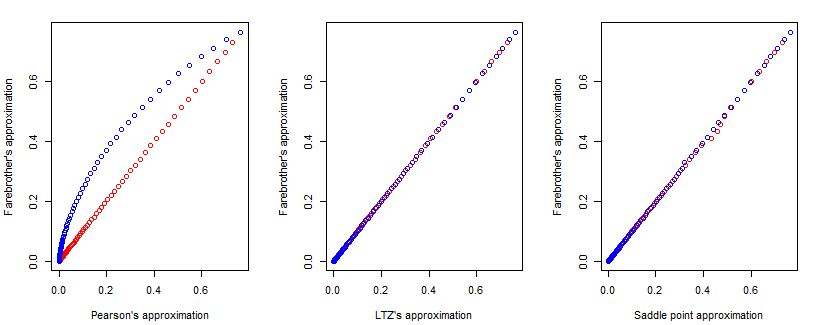
\includegraphics[width=\textwidth]{Q1&Q4}
		\title{Figure 4: qq plot of $Q_1$(red points) and $Q_4$(blue points)}
	\end{center}
\end{figure}
%\begin{figure}[h]
	\begin{center}
	%	\graphicspath{{C:/Users/riyi/Desktop/yusha/STAT-5123/project}}
%		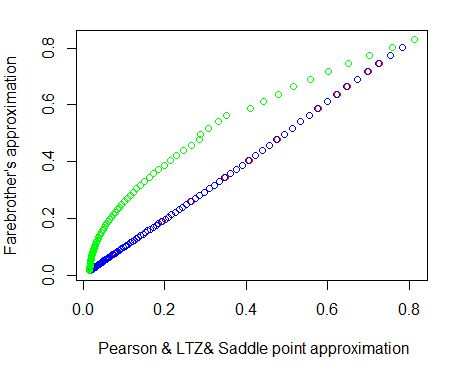
\includegraphics[scale=0.45]{Q5}\\
		
		\title{Figure 5: qq plot of $Q_5$: Pearson-red points, LTZ-blue dots, Saddle point-green dots}
	\end{center}
%\end{figure}

\clearpage
\section{Conclusion}
Our numerical results suggest that Farebrother's method and Imhof's method differ very little. Pearson's method is not appliable when the quantity of chi-square terms is large. Saddle point approximation performs well as a whole. LTZ's method perfoms much better compared to Pearson's method and it is the most accuracy except the Imhof's method. This method shows great advantage especially if the matrix A is complex and high-dimensional and thus has great realistic meaning. 

\end{document}
